%!TEX root =  ../main.tex

\subsection{Graphs}

\objective{Graph arbitrary power functions by hand}


\index{power function!graphs}
What is the simplest rational exponent function to graph?  $f(x)=x^1$, because $1=\frac{1}{1}$!  
1 is the identity of multiplication, and powers --- as groups of multiplication --- all go through
it.  Every graph of the type $f(x)=x^{\frac{m}{n}}$ passes through $(1,1)$.  In this section, we will
discuss how to graph any function of this type, but you must be sure that $\frac{m}{n}$ is a fraction
in simplest form (i.e. no common factors).

\subsection{Behavior $<1$}
Pick a number.  Square it.  Did it get bigger or smaller?  Bigger, of course, you say.  Well, 
that assumes you picked a number bigger than 1.  What would have happened if you had
picked a number $(0,1)$?  What is $0.5^2$?  $0.1^2$?  They both get smaller, 0.25 and 0.01
respectively.  


\begin{derivation}{Small Exponents and Small Numbers}
Size of the exponent will shape the graph
differently between $(0,1)$ than it will $(1,\infty)$.
\begin{itemize}
\item For $\frac{m}{n}>1$, $b^\frac{m}{n}$ will increase \emph{more} rapidly if $b>1$ and less rapidly  if $0<b<1$.\\
\item For $\frac{m}{n}<1$, $b^\frac{m}{n}$ will increase \emph{less} rapidly if $b<1$ and more rapidly if $0<b<1$.
\end{itemize}
\end{derivation}


So, if small exponents grow quickly to 1, and then slow down, while large exponents grow
slowly towards 1 and then quickly afterwards, we may broadly sketch graphs.

\begin{figure}
\begin{centering}
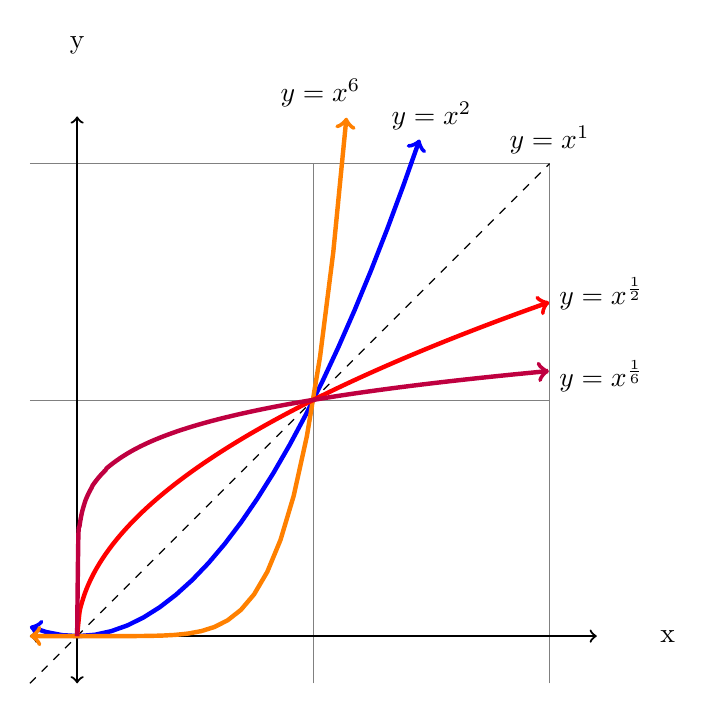
\begin{tikzpicture}[scale=3]
	\draw [help lines] (-0.2, -0.2) grid (2, 2);
	\draw [thick,<->] (-.2, 0) -- (2.2, 0);
	\draw [thick,<->] (0, -.2) -- (0, 2.2);
        % x-axis label
        \node at (2.5, 0) {x};
        % y-axis label
        \node at (0, 2.5) {y};

        \draw[dashed, -] (-.2,-.2) -- (2,2) node [anchor=south] {$y=x^1$};

        \draw[domain=-.2:1.45,<->,ultra thick,blue] plot (\x,\x*\x);
	\node at (1.5,2.1) [anchor=south] {$y=x^2$};

        \draw[domain=-.2:1.14,<->,ultra thick,orange] plot (\x,\x*\x*\x*\x*\x*\x);
	\node at (1.03,2.2) [anchor=south] {$y=x^6$};

        \draw[domain=0:2,->,ultra thick,red,samples=200,smooth] plot (\x,{sqrt(\x)});
	\node at (2,1.45) [anchor=west] {$y=x^{\frac{1}{2}}$};

        \draw[domain=0:2,->,ultra thick,purple,samples=400,smooth] plot (\x,{(\x)^(1/6)});
	\node at (2,1.1) [anchor=west] {$y=x^{\frac{1}{6}}$};
\end{tikzpicture}
\caption{Various power function graphs with exponents more and less than 1}
\end{centering}
\end{figure}

\subsection{Even, Odd, and Negative}
If the functions we are graphing are all of the type $f(x)=x^\frac{m}{n}$, then there will be
obvious patterns dependent upon what kind of numbers $m$ and $n$ are.  

\paragraph{$n$ is odd}
If the root we are taken is odd, then it is easily defined for both positive and negative real input,
so the function will exist across the entire real domain.  In other words, there will be both a
left and right half.

\paragraph{$n$ is even}
If the root we are taken is even, then negative inputs will be undefined.  Notice that this leads to
the major exception to our rule mentioned previously, that rational exponents are strictly equivalent
to powers over roots.  $\sqrt[4]{x^2}$ will work for negative inputs, but $x^\frac{1}{2}$ will not.

\paragraph{$\frac{m}{n}$ is negative}
When an exponent is negative, that is equivalent to a positive exponent in the denominator.
These reciprocal transformations were covered in chapter 4.
